\subsection{Estudo de técnicas de reconhecimento} 

As informações de distância recebidas pelos sensores descritos na seção
anterior podem ser armazenados como uma estrutura de dados chamada nuvem de
pontos, isto é, uma representação tridimensional do espaço cartesiano, na qual cada distância medida pelos
sensores a partir de sua origem representa uma coordenada x y z.
Entretanto, essa representação não é capaz de diferenciar, ou classificar, os
limites de cada objeto presente na cena, ou seja, não é possível determinar
\textit{a priori} qual conjunto de pontos pertence a cada elemento que se deseja
identificar para realizar a calibração.

A identificação de cada conjunto, ou \textit{cluster}, de pontos é importante
para que a posição e orientação de cada objeto de interesse seja determinada e,
assim a transformação do sistema de coordenadas entre cada objeto seja
calculada. Esse processo necessita, então, do estudo e implementação de
algoritmos para a análise da nuvem de pontos, identificação dos elementos
necessários, extração de suas respectivas posições e, finalmente, cálculo da
transformação entre as posições. 

Dependendo das características de cada objeto a ser identificado e da
possibilidade de implementação de uma estrutura de apoio para facilitar a sua
identificação, podem ser utilizados diferentes métodos e estratégias de
identificação e localização, que serão exploradas a seguir.

\subsubsection{Reconhecimento do Robô}

O Robô é uma estrutura que a idenficação pode ser facilitada pelo uso de
padrões de fácil reconhecimento (como esferas e padrões de xadrez, figuras
\ref{fig::sphere_rec} e \ref{fig::checkerboard_rec} ), pois alterações na base
do robô não ocasionam problemas para o funcionamento do sistema.


\begin{figure}[h!]
   \centering
   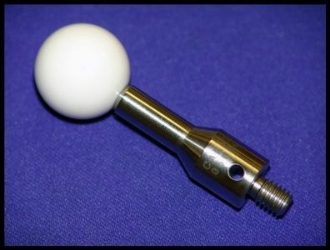
\includegraphics[width=0.95\columnwidth]{figs/localizacao/sphere_rec}
   \caption{Exemplo de esfera utilizada para reconhecimento. Fonte:
   http://shop.talwin.net/}
   \label{fig::sphere_rec}
\end{figure}



\begin{figure}[h!]
   \centering
   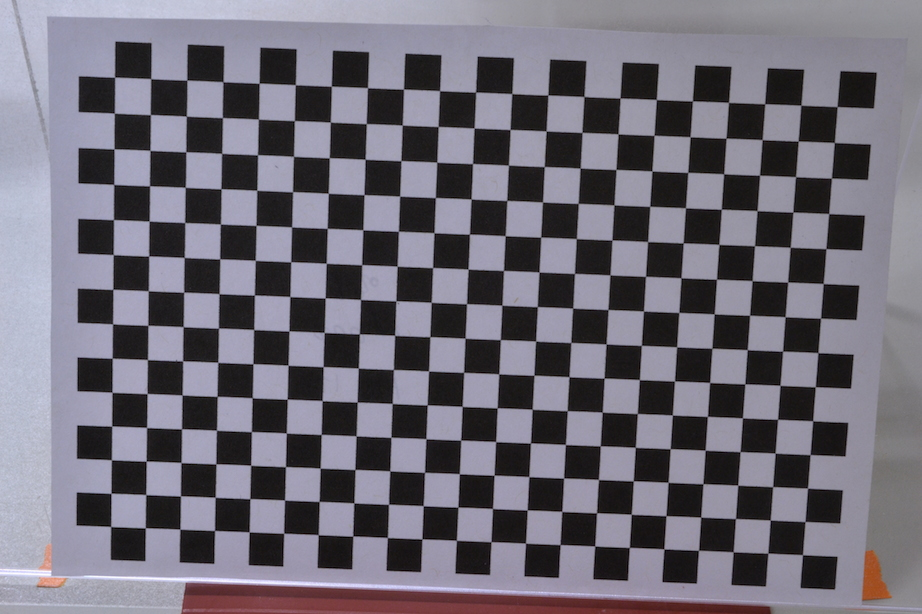
\includegraphics[width=0.95\columnwidth]{figs/localizacao/checkerboard_rec}
   \caption{Exemplo de padrão de xadrez utilizado para renhecimento.\\ Fonte:
   http://stereomorph.blogspot.com.br/}
   \label{fig::checkerboard_rec}
\end{figure}


Devido a baixa iluminação ambiente dentro do circui\-to da tubina, a opção
mais simples é o uso de nu\-vem de pontos sem identificação de cor. Ou seja, o
reconhecimento se dará apenas pelo formato. Isso restringe o uso de padrões de
xadrez e o foco se voltará, então, para o uso de formatos geométricos. Em
especial o mais simples objeto de três dimensões: a esfera.

O reconhecimento de formas geométricas simples em três dimensões é um assunto
já razoavelmente explorado na literatura. Dentre eles pode-se destacar 2
métodos: RANSAC e Hough Transform.

\paragraph{RANSAC}
O método RANSAC (acrônimo para ``RANdom SAmple Consensus", \textit{consenso por
amostragem aleatória} em tradução livre) é um método iterativo que tem como
premissa a presença de \textit{outliers} (elementos fora do corpo principal) na
amostra e objetiva a identificação dos parâmetros matemáticos que descrevem o
objeto geométrico em questão \cite{ransac}. É o método
disponível na amplamente utilizada biblioteca de processamento de nuvem de pontos ``PCL''. 

Esse método consiste na seleção aleatória de pontos para serem considerados como
partes integrantes do corpo principal (no caso, uma esfera), a partir desses os
parâmetros da esfera são calculados (comumente, os valores x, y e z do centro
da esfera e seu raio). Então os demais pontos são julgados como fazendo parte ou
não da esfera de acordo com esses parâmetros. O modelo é avaliado como bem estimado se uma quantidade razoável de pontos são considerados
como pertencentes à esfera. Se for visto como bem estimado, os parâmetros são
então reestimado levando em conta de todos os pontos que foram considerados como
pertencentes à esfera. O erro do modelo é inferido a partir dos pontos que foram
considerados como fazendo parte da esfera e uma esfera reconstruída pelos
parâmetros calculados. O processo então é repetido um número artrário de vezes,
e se mantém armazenado o modelo que obteve menor erro.

Um dos principais pontos negativos do RANSAC é que ele tem como premissa a
presença de apenas um corpo principal, ou seja, apenas uma esfera. Isso implica
em um tratamento especial quando temos mais de uma esfera no ambiente.

\begin{figure}[h!]
   \centering
   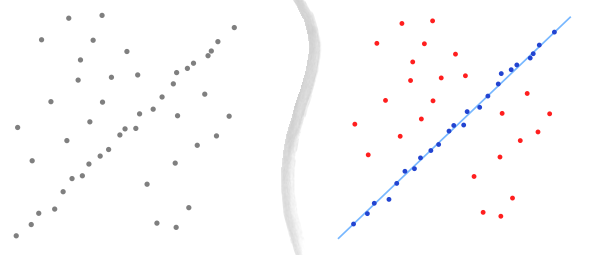
\includegraphics[width=0.95\columnwidth]{figs/localizacao/ransac}
   \caption{Exemplo de reconhecimento de uma linha em 2 dimensões usando
   RANSAC. (Fonte: \cite{ransac})}
   \label{fig::ransac}
\end{figure}
 
 \paragraph{Transformada de Hough 3D}
Anos de pesquisa em reconhecimento de objetos geométricos de duas dimensões
levaram ao desenvolvimento e aprimoramento de técnicas basedas em ``Transformada
de Hough''. Essas técnicas tem sido recentemente adaptadas para o universo de
três dimensões (ver \cite{hough2014}) e adequadamente chamadas de Transformada
de Hough 3D.

O método consiste em tranformar cada ponto do espaço 3D em uma variedade
mergulhada no espaço quadridimensional dos parâmetros da esfera ( x, y e z do
centro mais r do raio). A variedade se identifica com todas as possiveis esferas
que contém aquele ponto. O espaço de parâmetros é então restrito dentro de
certos limites e quantizado por razões de implementação (os recursos
computacionais são finitos). É definido então um acumulador, basicamente uma
função que conta quantas variedade interceptam determinada região discretizada
do espaço de parâmetros. Um algorítmo de reconhecimento de picos é aplicado
sobre o espaço de parâmetros (com as varidade já mergulhadas nele) para detectar
qual o conjunto de parâmetros que está melhor descrevendo um maior número de
pontos. O algorítmo pode ser utilizado para reconhecer mais de um pico e, assim,
identificar a presença de mais de uma esfera na nuvem de pontos (exemplo na
figura \ref{fig::hough}).

A dificuldade no uso do método é seu custo computacional, mas existem soluções
que exploram amostragens estatísticas para reduzir o custo computacional.

\begin{figure}[h!]
   \centering
   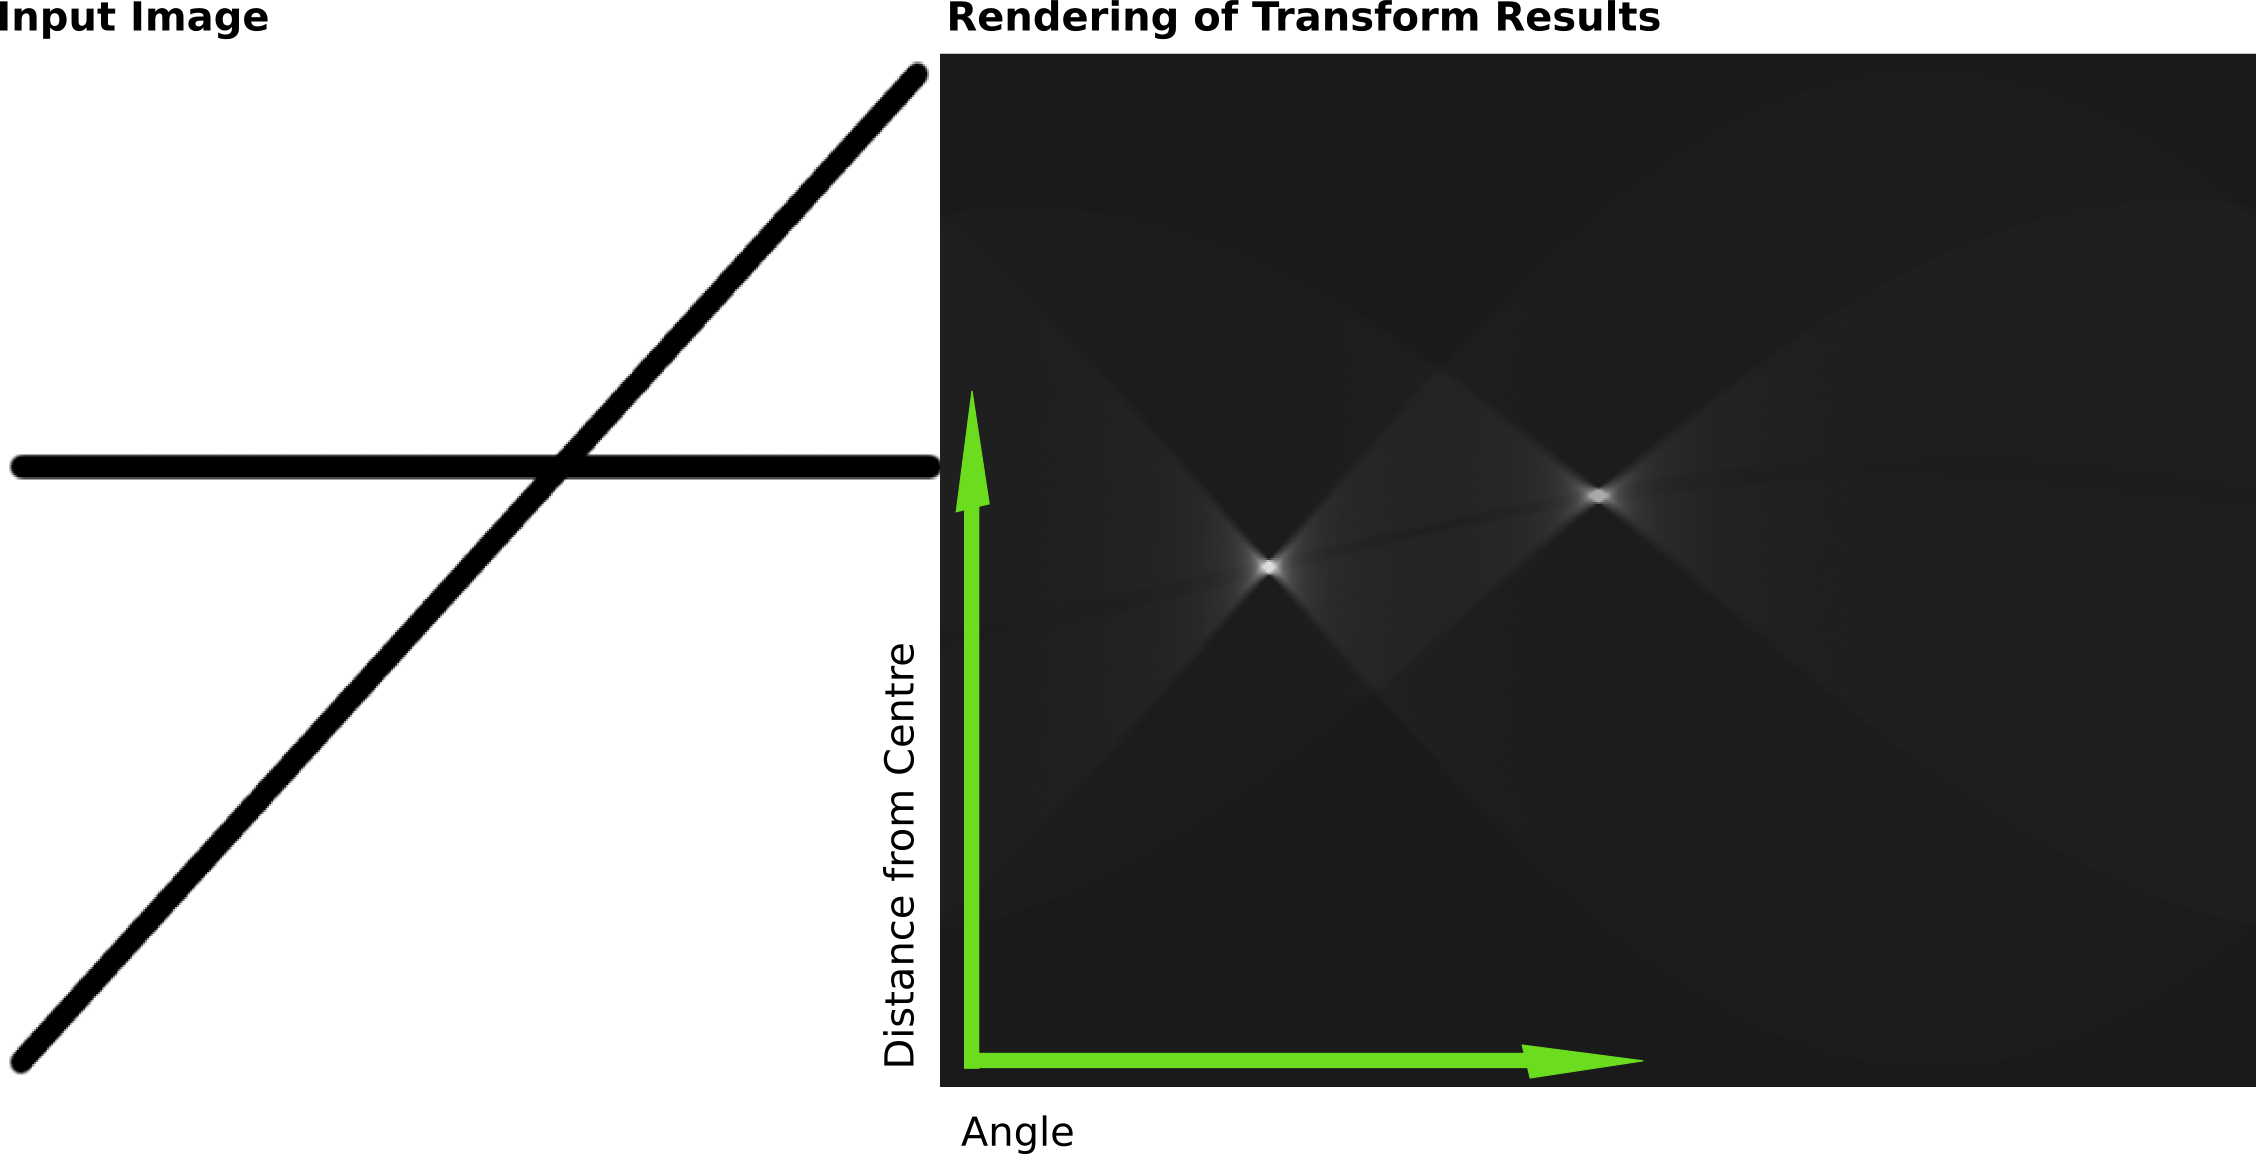
\includegraphics[width=0.95\columnwidth]{figs/localizacao/hough}
   \caption{Exemplo de reconhecimento de duas linhas em 2 dimensões usando
   Transformada de Hough. Na esquerda estão pontos que compõem as duas retas, na
   direita uma sobreposição das variedades referentes a cada ponto das retas
   (mergulhadas em um espaço paramétrico bidimensional). Os pontos mais
   brilhantes refletem os picos referentes aos parâmetros que melhor descrevem as duas retas. (Fonte: 
   \url{https://en.wikipedia.org/wiki/Hough_transform})}
   \label{fig::hough}
\end{figure}

Tendo conhecimento da posição de quatro esferas, pelo uso de um dos métodos
descritos acima, é possivel unicamente identificar a posição de um corpo preso a
elas. Em outras palavras, consegue-se a transformada entre origem do sistema de
coordenadas (tipicamente no sensor) e o robô. Para descobrir a trasnformada
entre o robô e a pá (posição relativa entre eles) falta identificar a
transformada entre a origem e a pá, esse caso será explorado na próxima seção a
seguir.

\subsubsection{Reconhecimento da Pá} 

Para a identificação e localização das pás das turbinas não é possível a
utilização de nenhum artifício de apoio que facilite o processamento da nuvem de
pontos, pois a instalação de qualquer um desses aparatos não pode ter precisão
garantida nas operações de campo. Uma instalação de um elemento de apoio em
pontos precisos da pá necessitaria também de calibração para cada utilização, retirando assim
o propósito do método. 

Portanto, para a localização das pás da turbina é
necessário explorar as características espaciais intrínsecas à superfície do
próprio objeto e identificá-las na nuvem de pontos do ambiente. O objetivo
principal nessa etapa do processo é, então, identificar um conjunto mínimo de
características do objeto que o represente unicamente com um baixo grau
de ambiguidade e sem exigir muito esforço computacional. 

A escolha do tipo de característica a se usar é uma decisão fundamental para a
eficiência do processo e tem sido alvo de estudos na literatura para a análise
e reconhecimento de imagens 2D, como imagens RGB de câmeras e mais recentemente
também para imagens 3D. 

Uma boa representação de \textit{point feature} deve ser capaz de capturar as
mesmas características locais da superfície na presença de:

\begin{itemize}
  \item \textbf{Transformadas} -  rotações e translações 3D nos dados não devem
  influenciar a estimação dos descriptors;
  \item \textbf{Variações na densidade de amostragem} - em princípio, uma de
  superfície amostrada mais ou menos densamente deve ter a mesma assinatura característica do vetor
  \item \textbf{Ruído}
\end{itemize}

O reconhecimento de objetos em aplicações robóticas também vem recebido
grande atenção, principamente com o crescimento da robótica móvel e em ambientes
não estruturados, onde é necessário identificar e localizar os objetos a serem
manipulados em cada tarefa. O problema é enfrentado basicamente utilizando-se
duas abordagens: analisar os dados 3D ou realizar algum tipo de processamento e
projeção para se trabalhar com imagens 2D e utilizar as técnicas mais maduras
desse tipo de imagem.

Nesta última categoria, a técnica
mais usada consiste em converter as informações tridimensionais em \textit{Range
Images}, na qual é realizada uma projeção a partir de um ponto de vista (geralmente o do sensor) e utiliza escala
de cores ou cinza para representar a distância, ou seja, quanto mais escuro o
objeto na imagem, mais longe ele se encontra. É importante reassaltar que esse
tipo de método introduz perdas de informação ao se realizar projeções e é
sensível à escolha do ponto de vista escolhido. 
%Em \cite{Bayramoglu2010} são
%utilizados descritores SIFT, ou \textit{Scale-Invariant Feature Transform},  
%como características a serem identificadas na imagem. \textit{Local Feature
%Histograms} são utilizados em \cite{Hetzel2001} e por sua vez \cite{Chen2007}
%optou por utilizar \textit{Local surface patches}. 
A escolha do descritor a ser
utilizado depende da aplicação e deve ser estudada a melhor opção para a nossa
solução, assim que tivermos dados aquisitados pelo sensor. Aplicações
semelhantes envolvendo identificação de objetos no ambiente tridimensional, mas
sem localizá-los, e utilizando diferentes descritores podem ser encotradas em
\cite{Bayramoglu2010,Hetzel2001,Chen2007}. Uma comparação dos descritores
utilizados para reconhecimento de objetos 2D e 3D pode ser encontrado em \cite{Zaharia2004, Weber2014}.

Após o reconhecimento do objeto, é necessário identificar a sua posição.
Em \cite{Steder2009}, o alinhamento é realizado utilizando-se a própria
\textit{Range Image} e a informação de profundidade presente na mesma. Por outro
lado, em \cite{Nuchter2005} a região onde o objeto identificado está presente é
selecionada e, por meio de \textit{raycasting} o conjunto de pontos da nuvem
pertecentes à região identificada na \textit{Range Image} é reprojetado. Após
essa segmentação, é utilizado um algoritmo de alinhamento como o ICP.

O primeiro passo para tornar possível a localização da pá é a aquisição de seus
dados espacias e a criação de uma nuvem de pontos que a represente. A
figura \ref{fig::pa_pcd} ilustra uma nuvem de pontos representando uma pá de uma das
turbinas da usina de Jirau, esse modelo foi construído utilizando-se os dados
aquisitados durante a viagem de campo e teste de sensibilidade do sensor Faro
Focus X330, como citado anteriormente. É importante ressaltar que o
modelo deve representar, se possível, todas as características pertinentes do objeto de interesse. Nesse
sentido, se faz necessário a criação de um modelo para cada tipo de pá que
deverá ser processada, ou seja pás com diferentes perfis hidráulicos possuem
modelos diferentes.


\begin{figure}[h!]
   \centering
   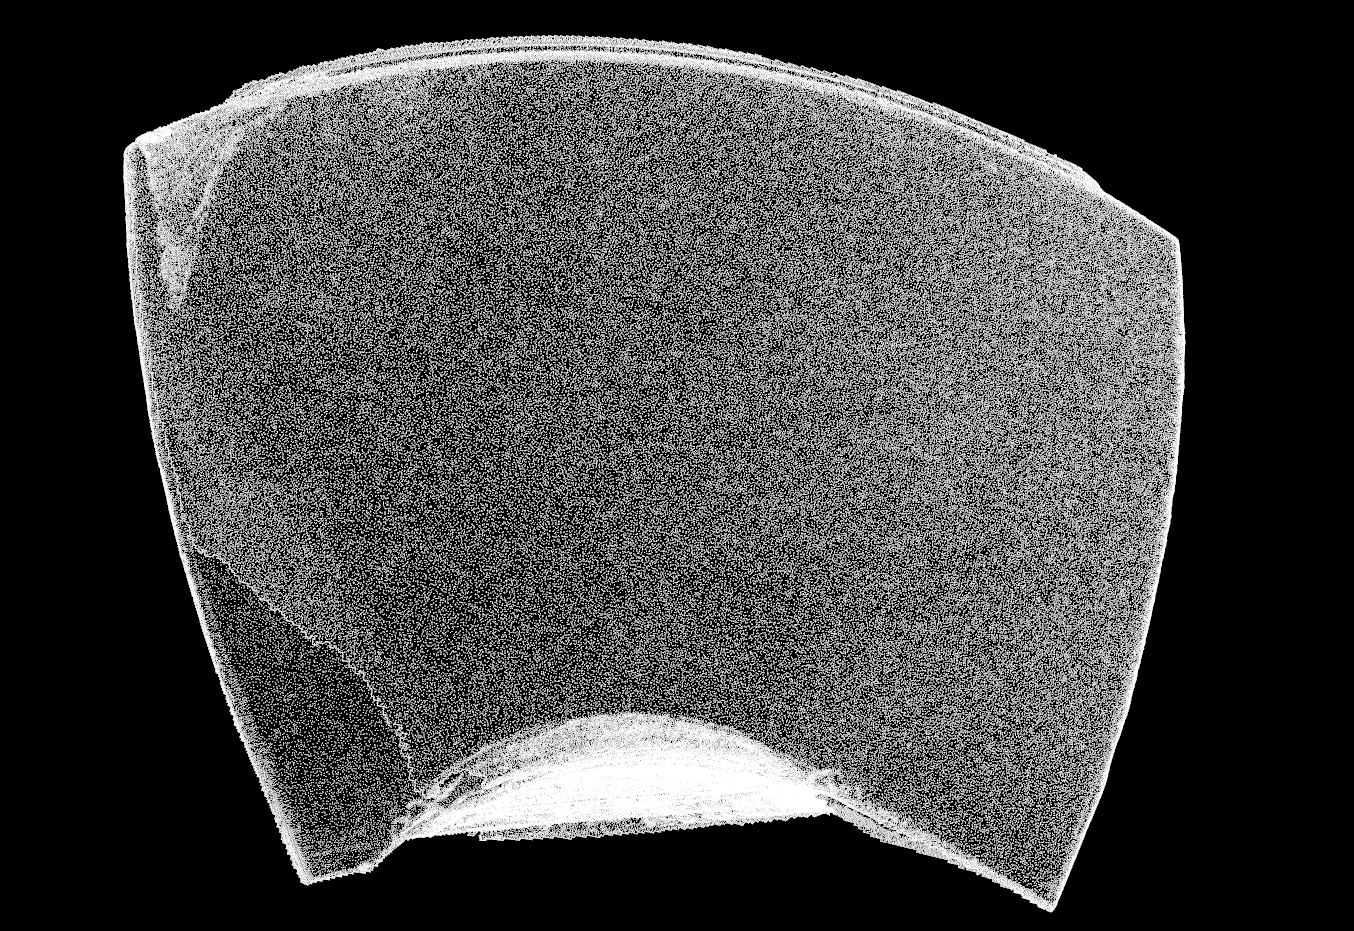
\includegraphics[width=0.95\columnwidth]{figs/localizacao/pa_pcd}
   \caption{Modelo da pá em nuvem de pontos}
   \label{fig::pa_pcd}
\end{figure}

A partir do modelo, é necessário a extração de seus pontos chaves e descritores.
A figura \ref{fig::pa_key} ilustra descritores do tipo SHOT, identificados no modelo de referência da pá. Para a nossa aplicação, não é
necessário, a princípio, o reconhecimento do objeto em questão, apenas a sua
localização e orientação no espaço tridimensional. A possibilidade de inserir no
sistema a informação de qual modelo de pá deve ser procurado, simplifica o
algoritmo e o torna menos suscetível a erros, uma vez que não é necessário
avaliar qual o modelo mais próximo das medições atuais e ainda é possível 
utilizar essa informação para fornecer uma avalição da similaridade do modelo
com os dados reais aquisitados.

\begin{figure}[h!]
   \centering
   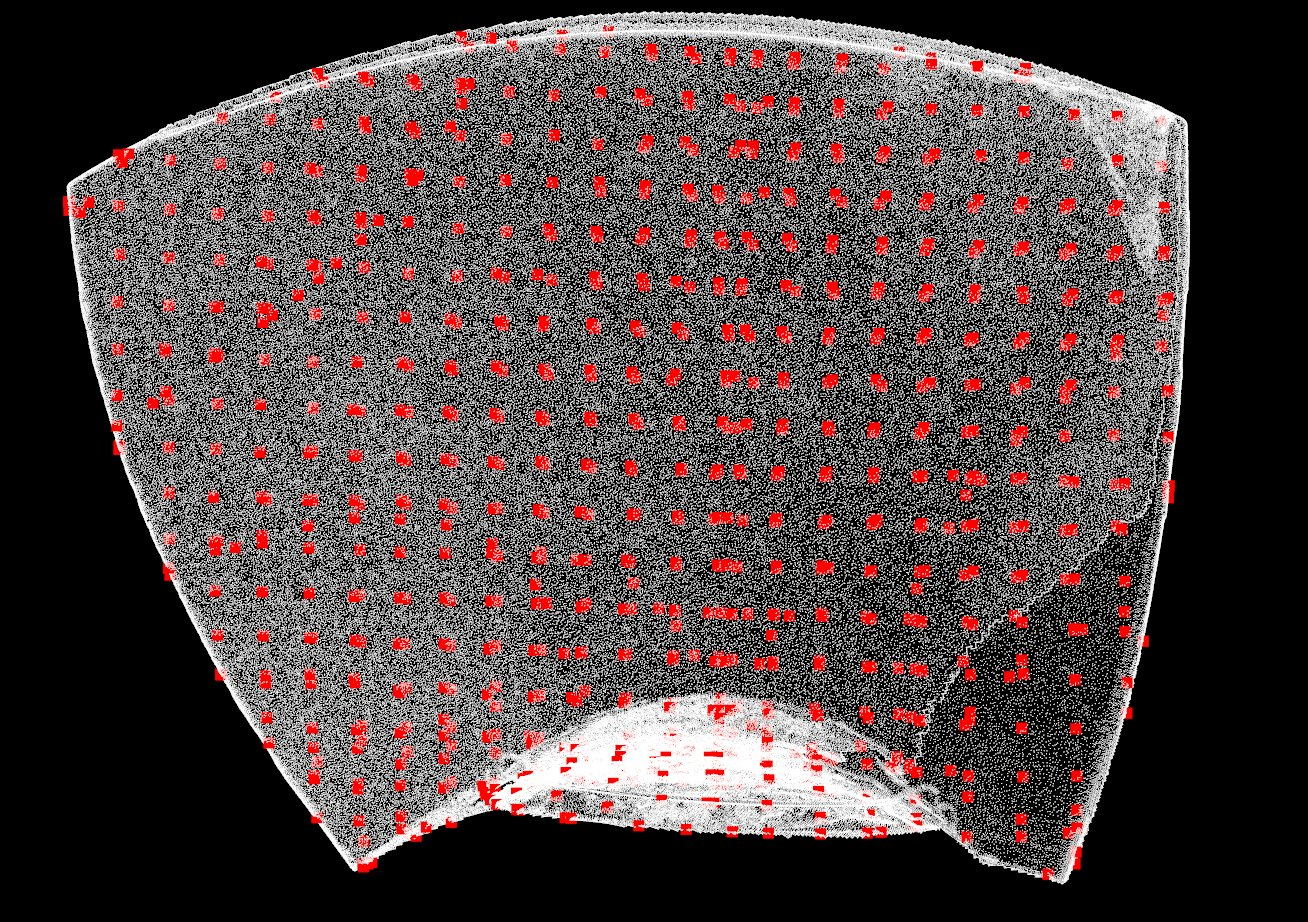
\includegraphics[width=0.95\columnwidth]{figs/localizacao/pa_key}
   \caption{Pontos de interesses com descritores associados no modelo da pá}
   \label{fig::pa_key}
\end{figure}

Uma vez que os pontos de interesse do modelo e seus descritores são extraídos, é
possível armazená-los para evitar o seu processamento  durante cada nova
calibração. Utilizando-se a estratérgia de
\textit{Correspondence Grouping} e o algoritmo \textit{Hough Voting}
\cite{Tombari2010a}, a nuvem de pontos aquisitada em campo terá também seus
pontos de interesse extraídos e um descritor associado para cada ponto. A
seguir, os descritores de ambas as nuvens, cena e modelo, são comparados afim de
se encontrar correpondentes em cada conjunto. Se um número suficiente de
correspondências é encontrado, o objeto é então detectado e localizado na
imagem. É importante ressaltar que essa técnica pode gerar falsos positivos. A
figura \ref{fig::correspondence} ilustra a implementação do algoritmo com 
dados sintéticos de uma cena, utilizando-se porém o modelo real da pá. O modelo
da pá está representado em amarelo, a pá identificada na cena em vermelho e as correspondências
conectadas pelas setas verdes.
Como próximos passos é necessário a utilização de dados reais para validação do
algoritmo e também a utilização de diferentes descritores, uma vez que apenas os
descritores do tipo SHOT foram testados.

\begin{figure}[h!]
   \centering
   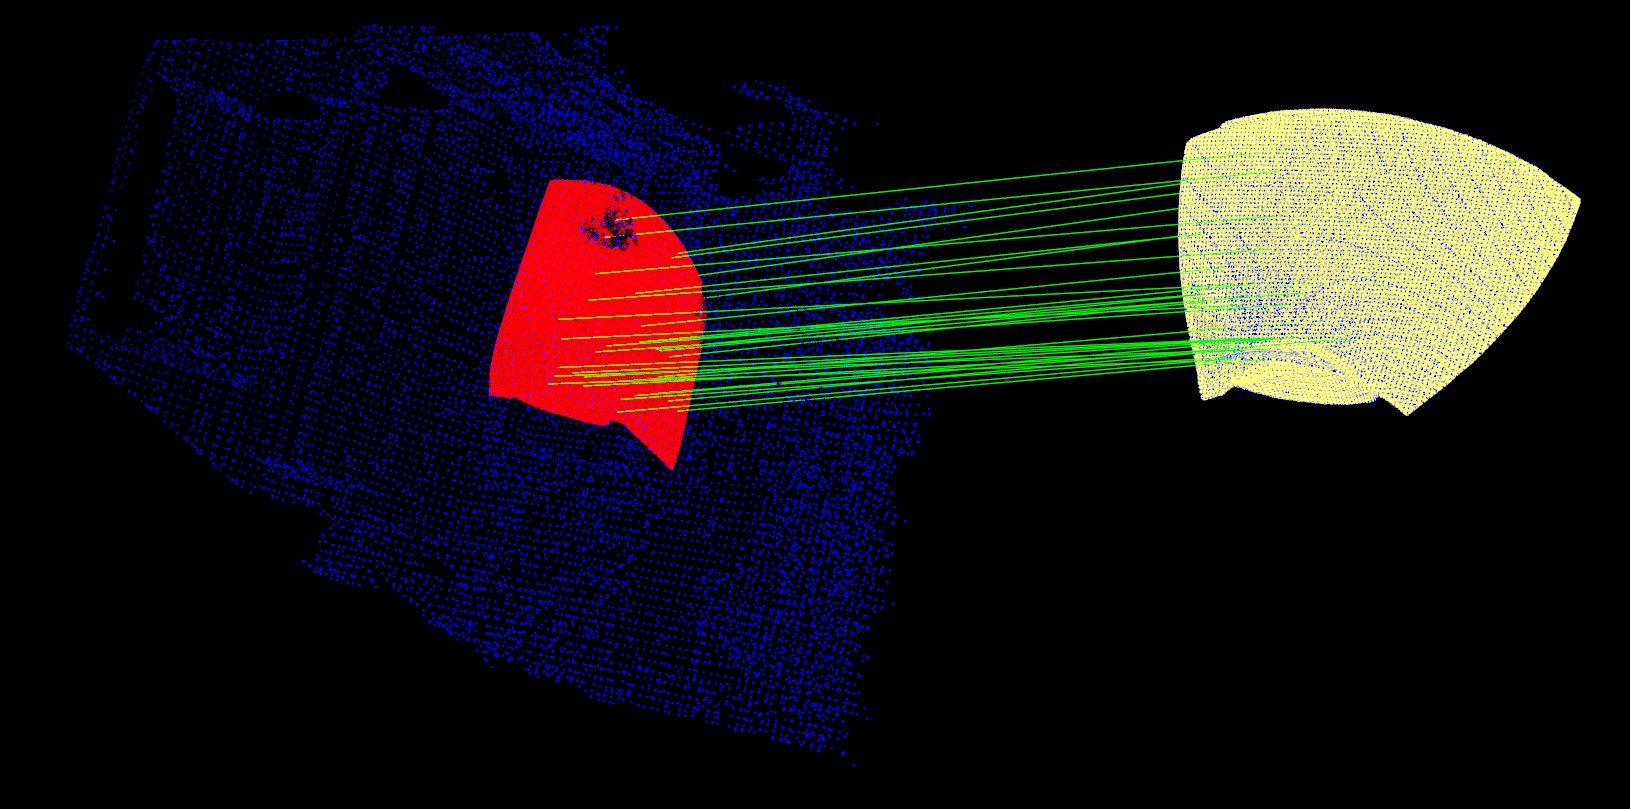
\includegraphics[width=0.99\columnwidth]{figs/localizacao/correspondence}
   \caption{Identificação e localização de uma pá utilizando
   \textit{Correspondence Grouping}}
   \label{fig::correspondence}
\end{figure}



